\documentclass[12pt]{article}
\usepackage{url}
\usepackage[margin=0.5in]{geometry}
\usepackage{graphicx}
\graphicspath{ {/}}


\title{Fairbook: USSA}

\author{A. Snow, C. McKenzie, C. Yang, J. Lyons, M. Zhang}

\begin{document}
	\maketitle


	\tableofcontents
	\section{ONIDs}
		snowan, mckencod, yangco, lyonsja, zhangm4



	\section{User Stories}
	\begin{enumerate}
	\item As a User I can search for textbooks by using different search criteria so that relevant results are returned. 

	\item As a User I can add textbooks to the cart so that I can keep track of the books I am interested in.

	\item As a User I can remove textbooks I no longer want from the cart.

	\item As a User I can log in so that I can access additional features (cart, ordering). 

	\item As a User I can edit my personal account information so that it is kept up to date. 

	\item As a User I can edit my payment information so that is is kept up to date. 

	\item As a User I can filter my searches (via author, title, keyword) so that the display of unwanted materials is minimal.

	\item As a User I can select a specific book so that I can view detailed information on it.

	\item As a User I can choose which seller I want to purchase a book from, so I can get the price and condition I want. 

	\item As a Seller I can list a book for sale including condition, price, access code status, and a picture so that the information is accurate.

	\item As a Seller I can manage my current listings and remove ones I no longer want.

	\item As a Manager I can delete/ban user accounts and edit user permissions.
	\end{enumerate}



	\section{Corresponding Tasks}
		\begin{enumerate}
		\item We need to set up a search box which let users type some keywords, and then the textbooks whose information contain the keywords will be shown. 
		This task can be worked with task 7 since they are both about searching. 
		It will take a pair of programmers about 2-3 hours to finish them. (future plan)
		\item When the user click the “add to cart” button for a specific textbook, that textbook should be added to the list called “cart”. 
		We should also make a class named “cart status” for each textbook, and give value “not-carted” initially. 
		After the textbook is carted, its “cart status” should change to “carted”. 
		When “add to cart” button is clicked, a check of “cart status” should happen in order to avoid repeat carting. 
		If the textbook is carted already, a warning window will show up; otherwise, just keep going. 
		It will take a pair of programmers 1-2 hours to finish. (next week)
		\item	In the cart, we can click the “remove from cart” button to remove the specific textbook from “cart” list. 
		Then the class “carted status” for that textbook should be changed to “not-carted”. 
		This task should be processed with task 2 since they are both about cart. 
		It should cost less than one more hour after task 2. (next week)
		\item	We should give access of carting, ordering, managing account information, and so on, to logged-in users only. 
		We will do some research online to add login section. 
		It will cost 2-3 hours, maybe more, to finish it, since we need to do some research to figure it out before work on it. 
		It would be better for us to process this task before task 2, 3, 5, 9, 10, since these operation all require access for login users. (future plan)
		\item	We should link personal account information to specific login user. 
		To change personal account information, we may need to do some research on how to use stripe.js. 
		It may cost 2-3 hours or more, and most of time should be used on searching and trailing.(possibly)
		\item Similar to task 5. After we finish task 5, we will spend less than one hour to finish this task.	
		\item	The other one is set up a filter, which users will check the property of the textbooks which they want to search. 
		Then the filter will show results according to the property checked which are stored as class name in the information of individual textbooks. 
		This task can be worked with task 1 since they are both about searching. 
		It will take a pair of programmers about 2-3 hours to finish them. (future plan)
		\item When users are viewing textbooks list, they are at “textbooks” page. 
		When they click on a specific book, it will redirect to the “textbook” page. 
		Then specific information store in classes will be shown, such as price, condition, area, and so on. 
		This task will take 1-2 hours to be done. (next week)	
		\item	In the “textbook” page, there should be a drop-down section which shows different sellers who are selling this book. 
		This should be processed after task 9 is finished. 
		It should take about 1-2 hours to be finished. (future plan)
		\item	In personal account page, we need to add to “sell your textbooks” button, which will call out a textbook information modal, which lets seller fill in the information of their textbooks.
		 After they confirm the information, this new selling textbook will be added in “textbooks” page following the already existing ones. 
		 Moreover, the new selling textbook will be stored under “selling” page in seller’s personal account. 
		 This task should be worked on after task 4, 5 and 6 are finished. 
		 It will take about 2 hours to make it finished. (future plan)
		\item	We will add an “edit” button for each listing textbook. 
		After seller clicks on it, the textbook information modal will be called out, but with existing information this time, different with the situation when seller wants to add a textbook. 
		After seller changes the information, new information will replace the old one simply. 
		This task should be worked on after task 10 is finished. 
		It may take us 2-3 hours. (future plan)
		\item	Whenever a new user is registered, it will be added to “user” list, which only manager has access to. 
		From this problem of authority, we need a lot of search to make it work, so I think we are going to spend 1 or 2 days on it. 
		This task can be done anytime, but just need to be done before our program is delivered to public/customers. (future plan)
			
		\end{enumerate}

	\section{UML Sequence Diagrams/Spikes}
		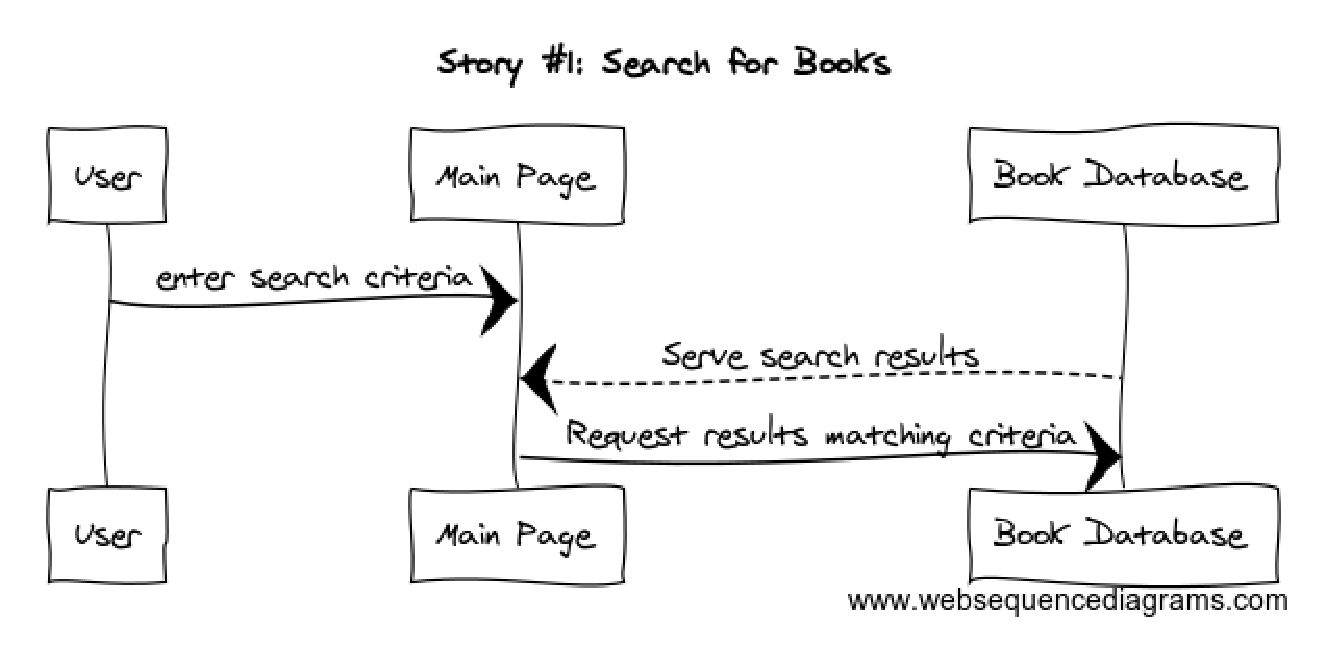
\includegraphics[width=16cm]{story1.eps}
		\par
		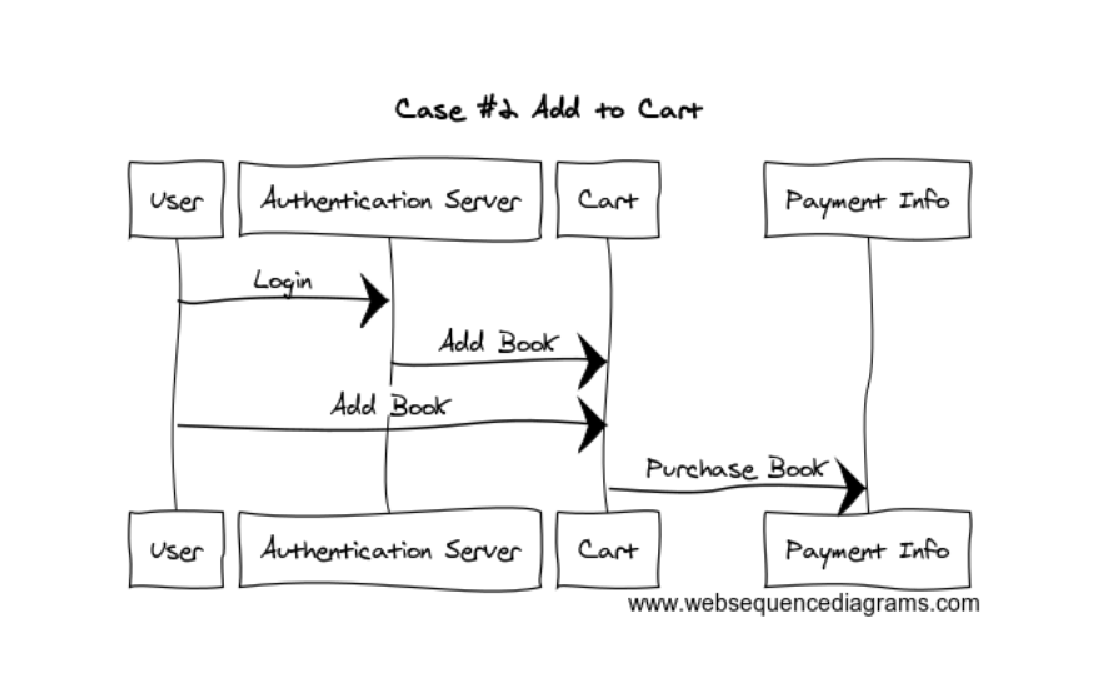
\includegraphics[width=14cm]{story2.eps}
		\par
		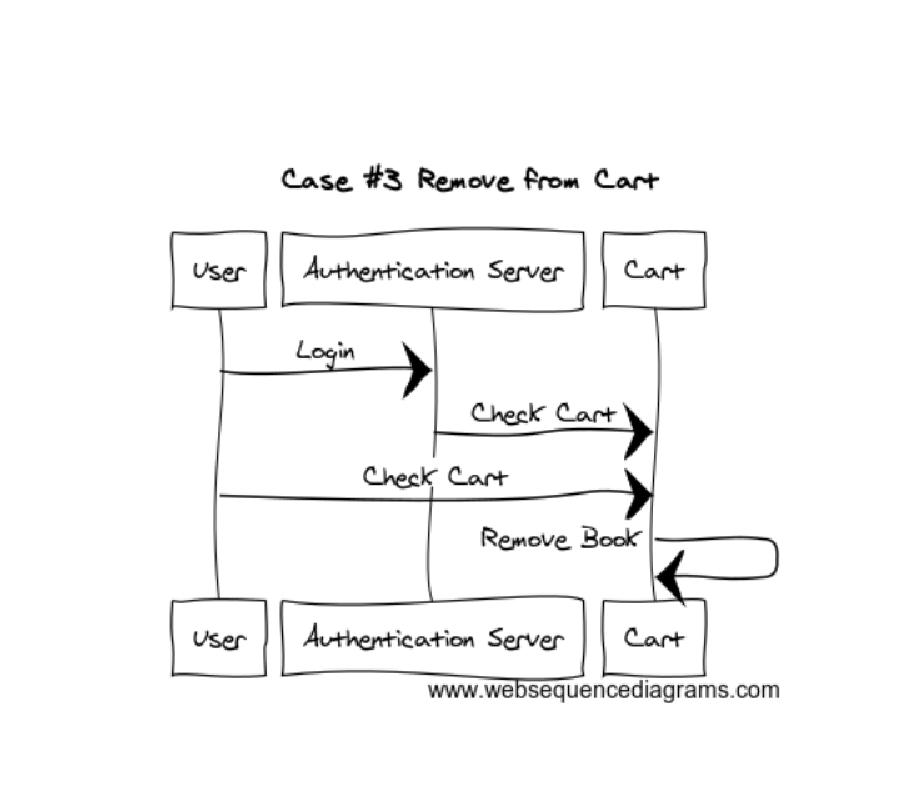
\includegraphics[width=12cm]{story3.eps}
		%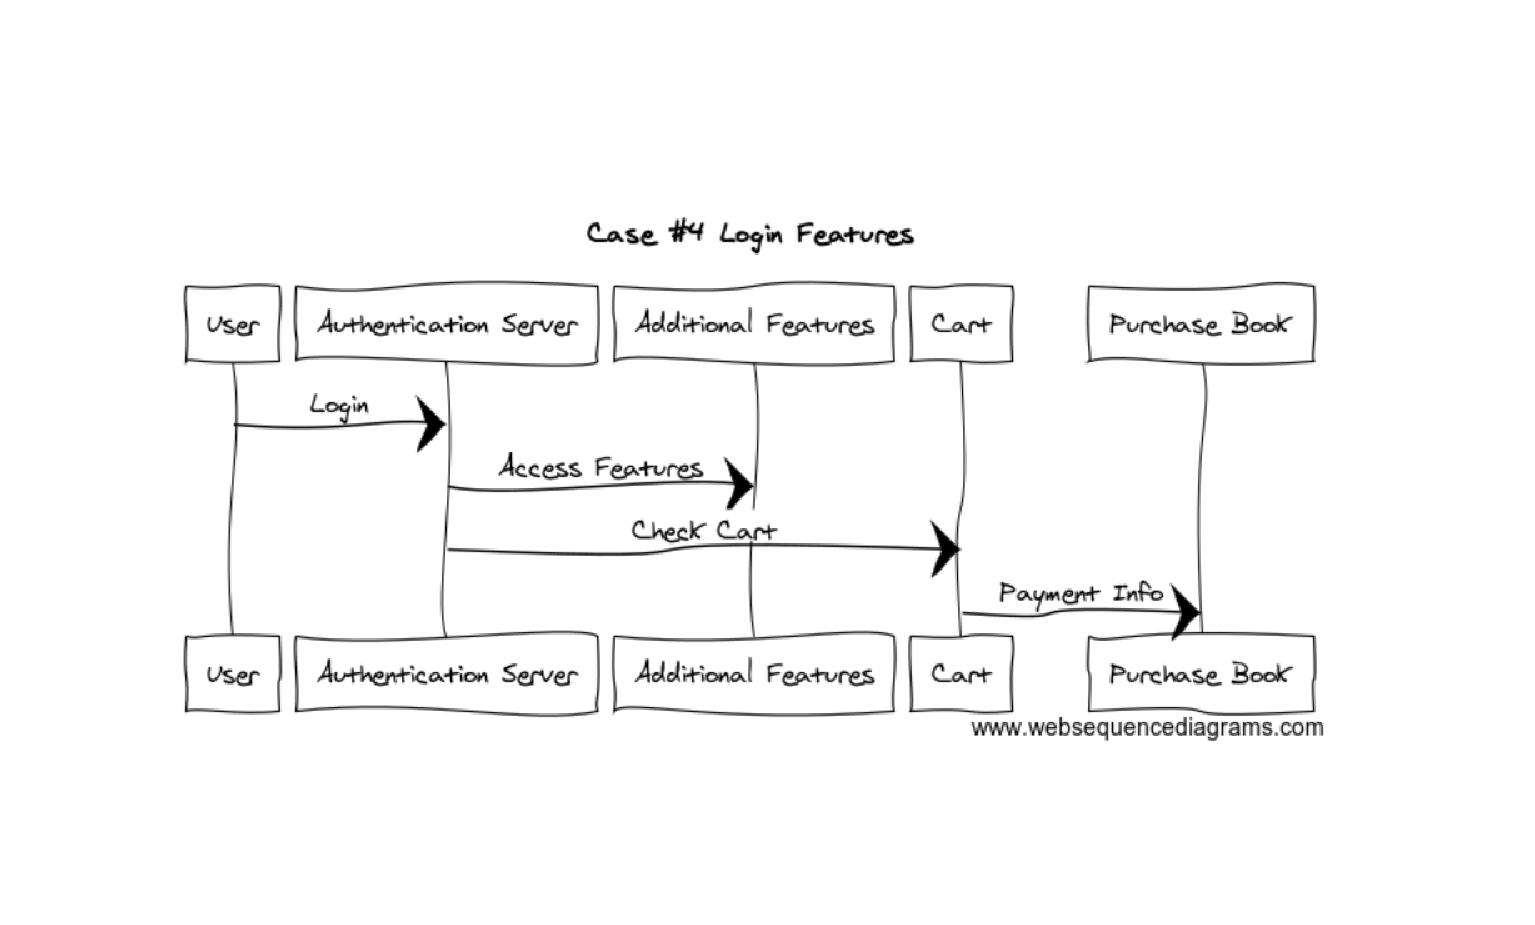
\includegraphics[width=16cm]{story4.eps}
		\par
		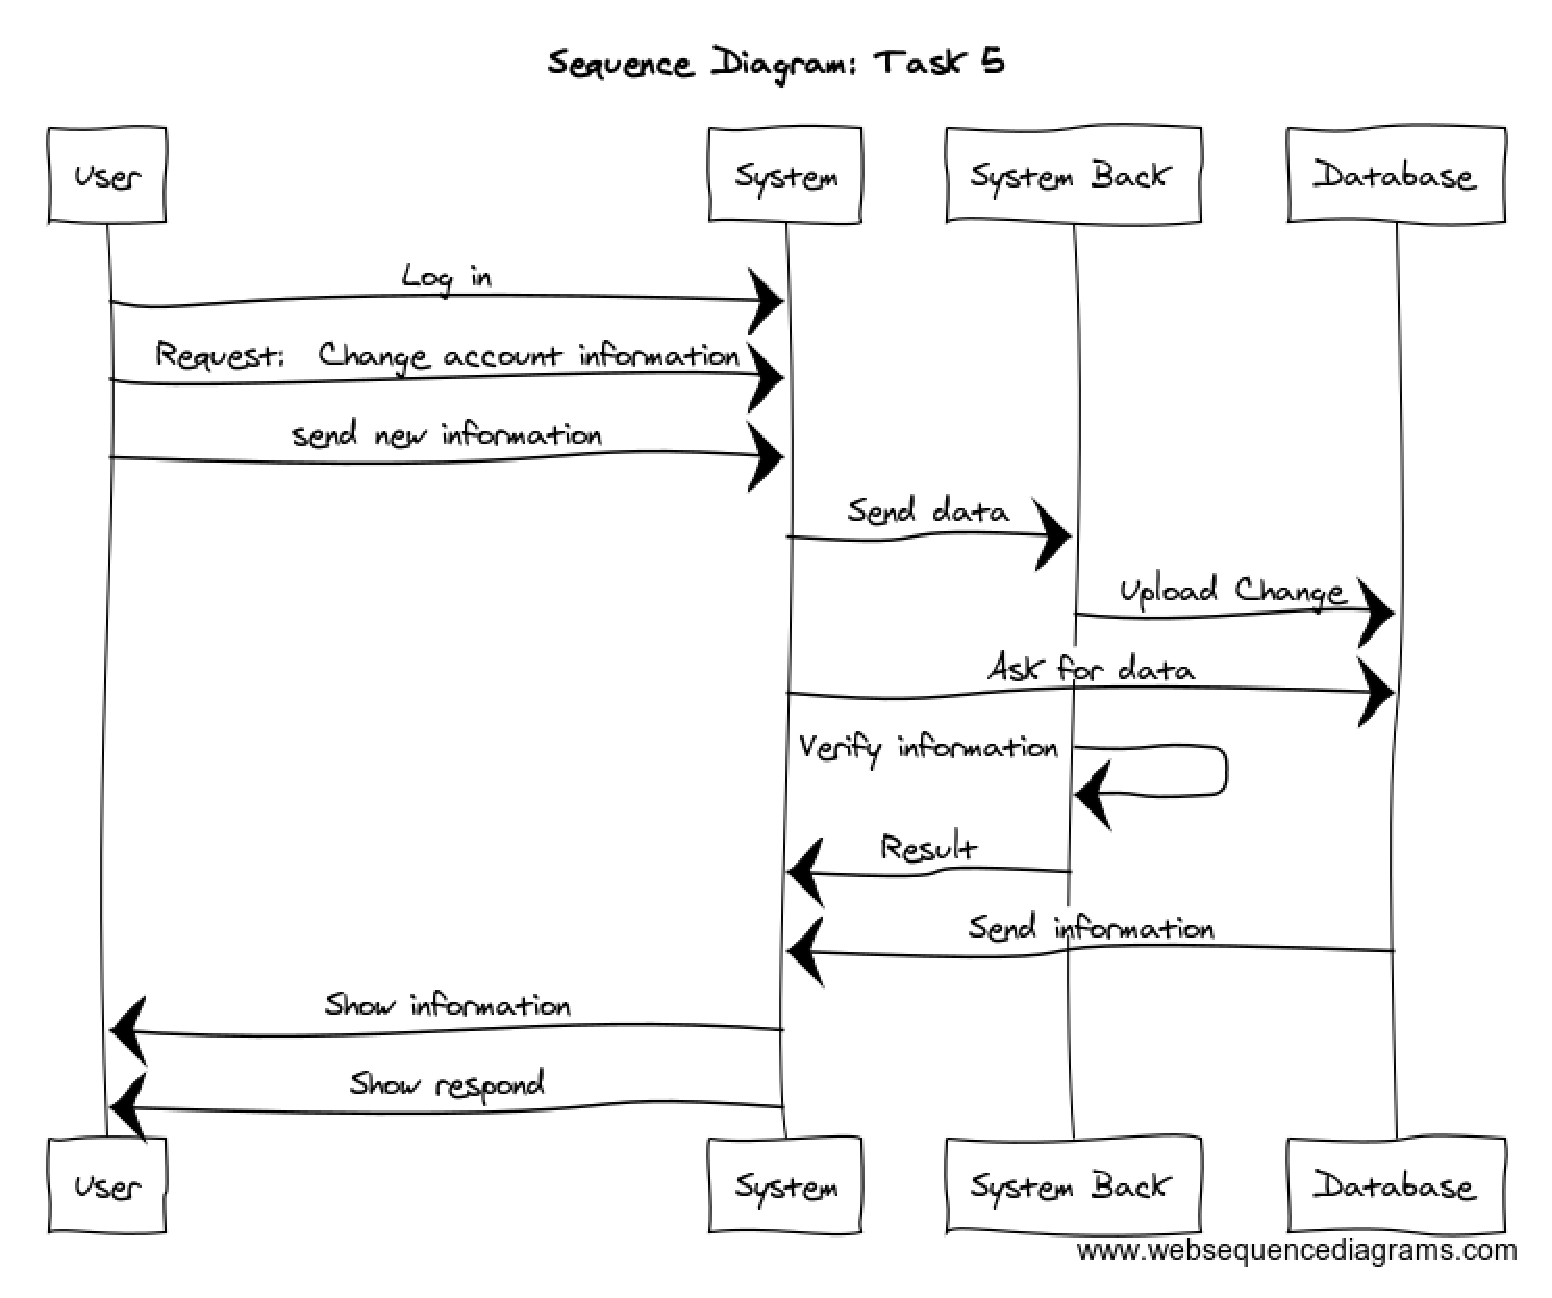
\includegraphics[width=16cm]{story5.eps}
		\par
		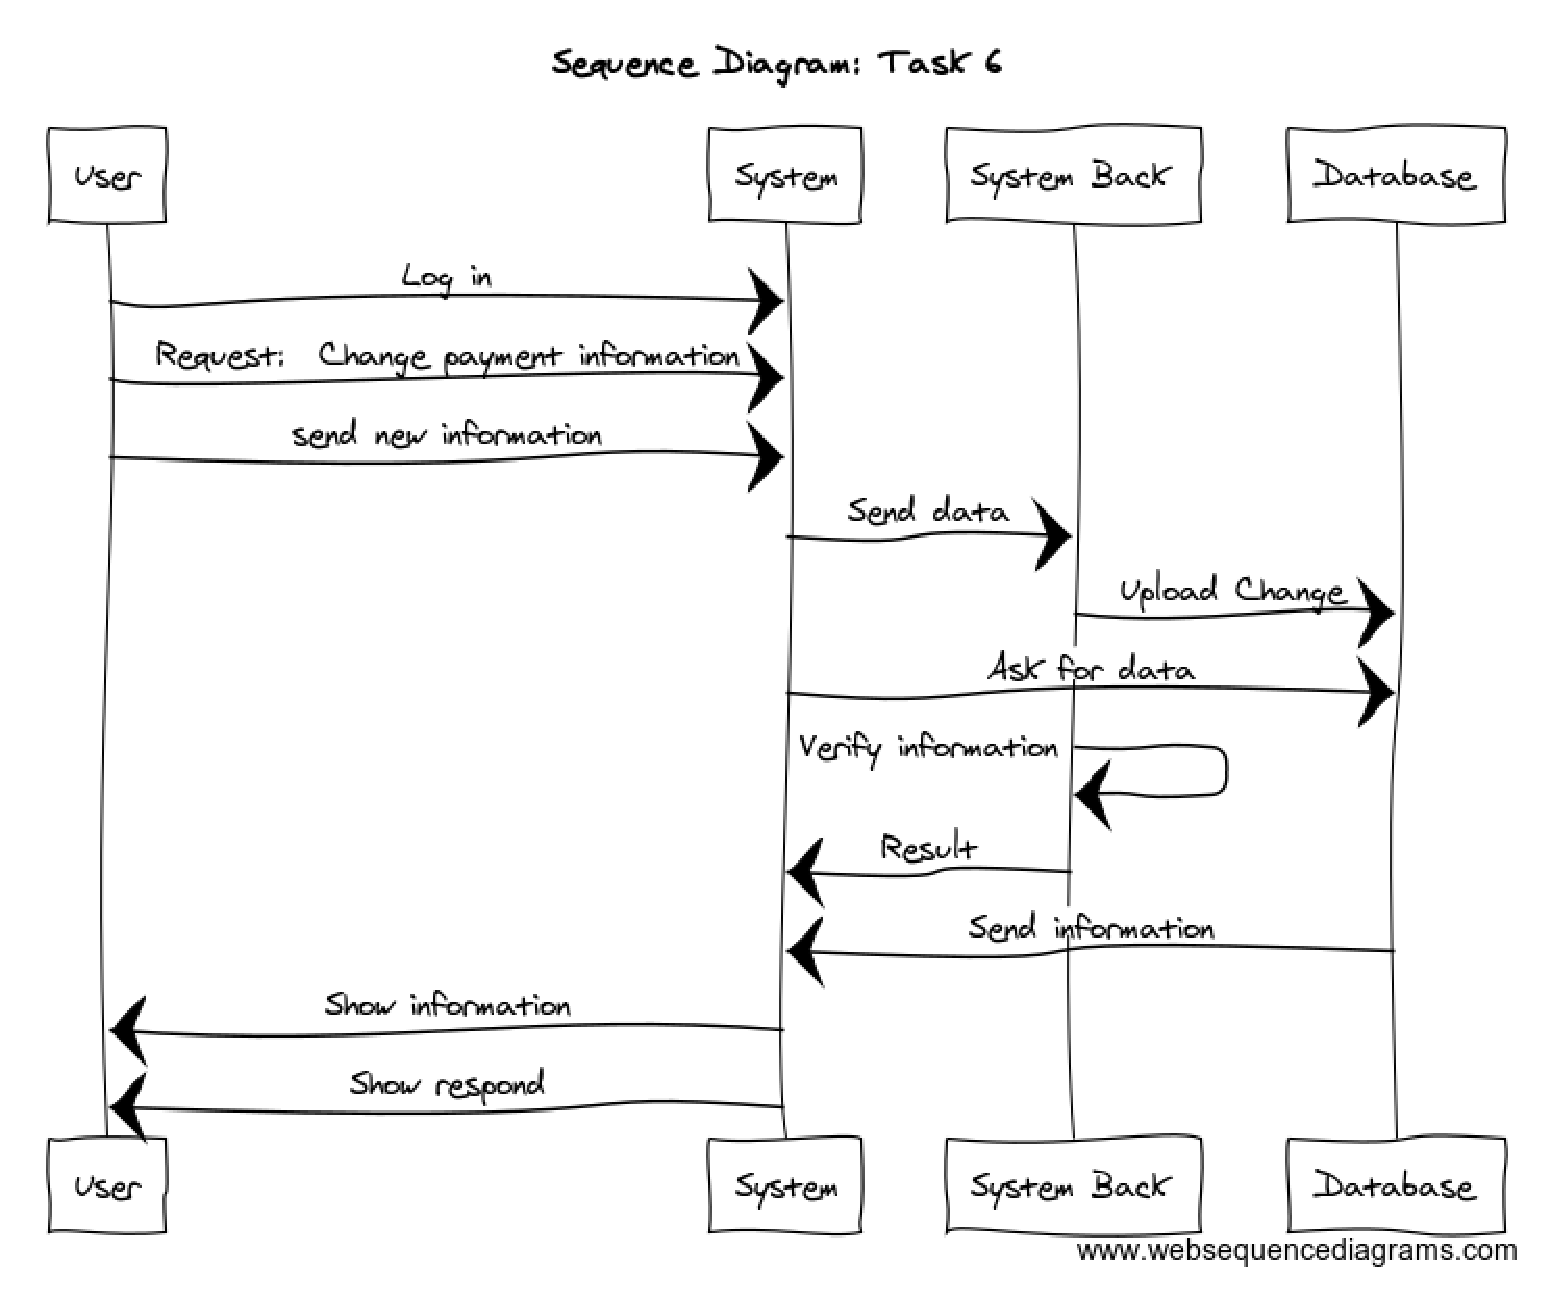
\includegraphics[width=16cm]{story6.eps}
		\clearpage
 		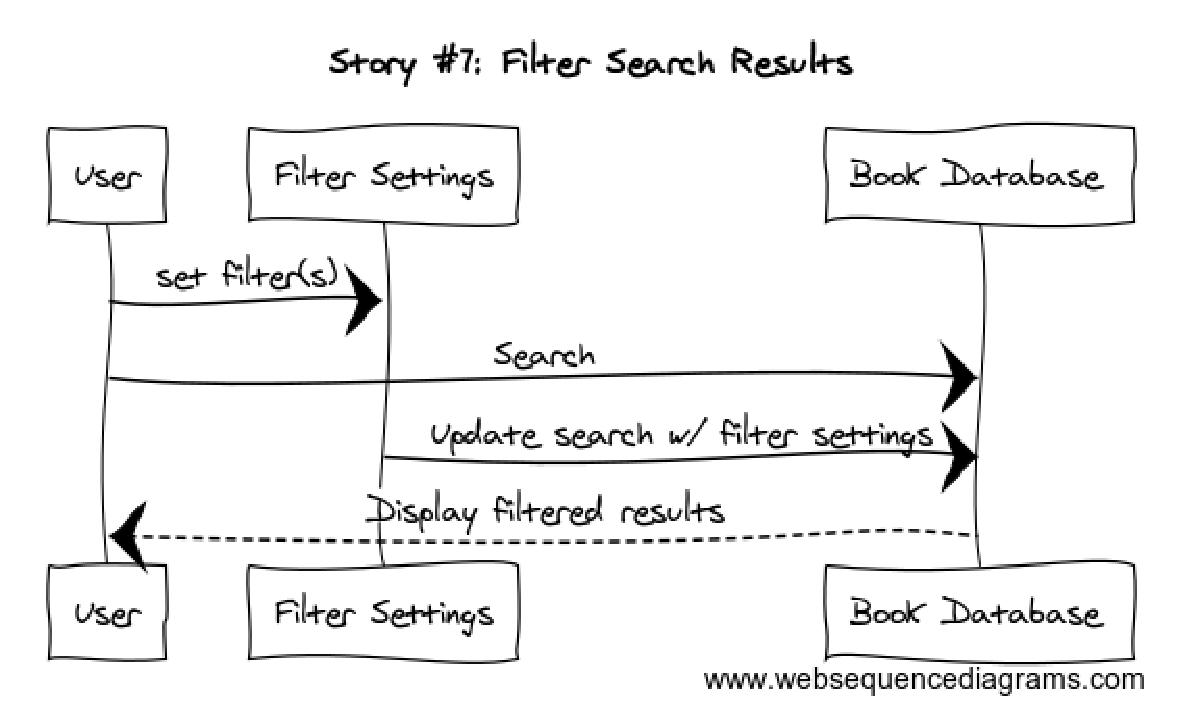
\includegraphics[width=16cm]{story7.eps}
 		\clearpage
 		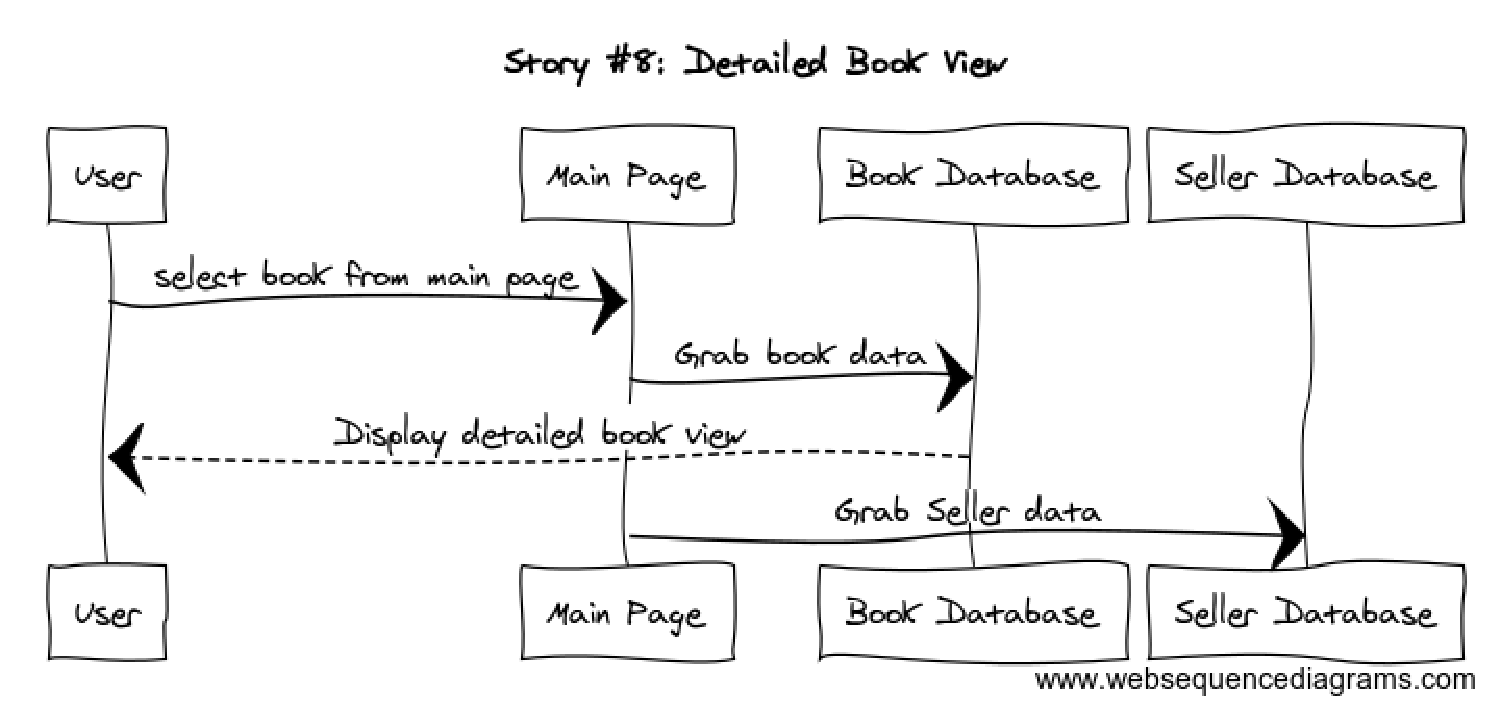
\includegraphics[width=16cm]{story8.eps}
 		\clearpage
 		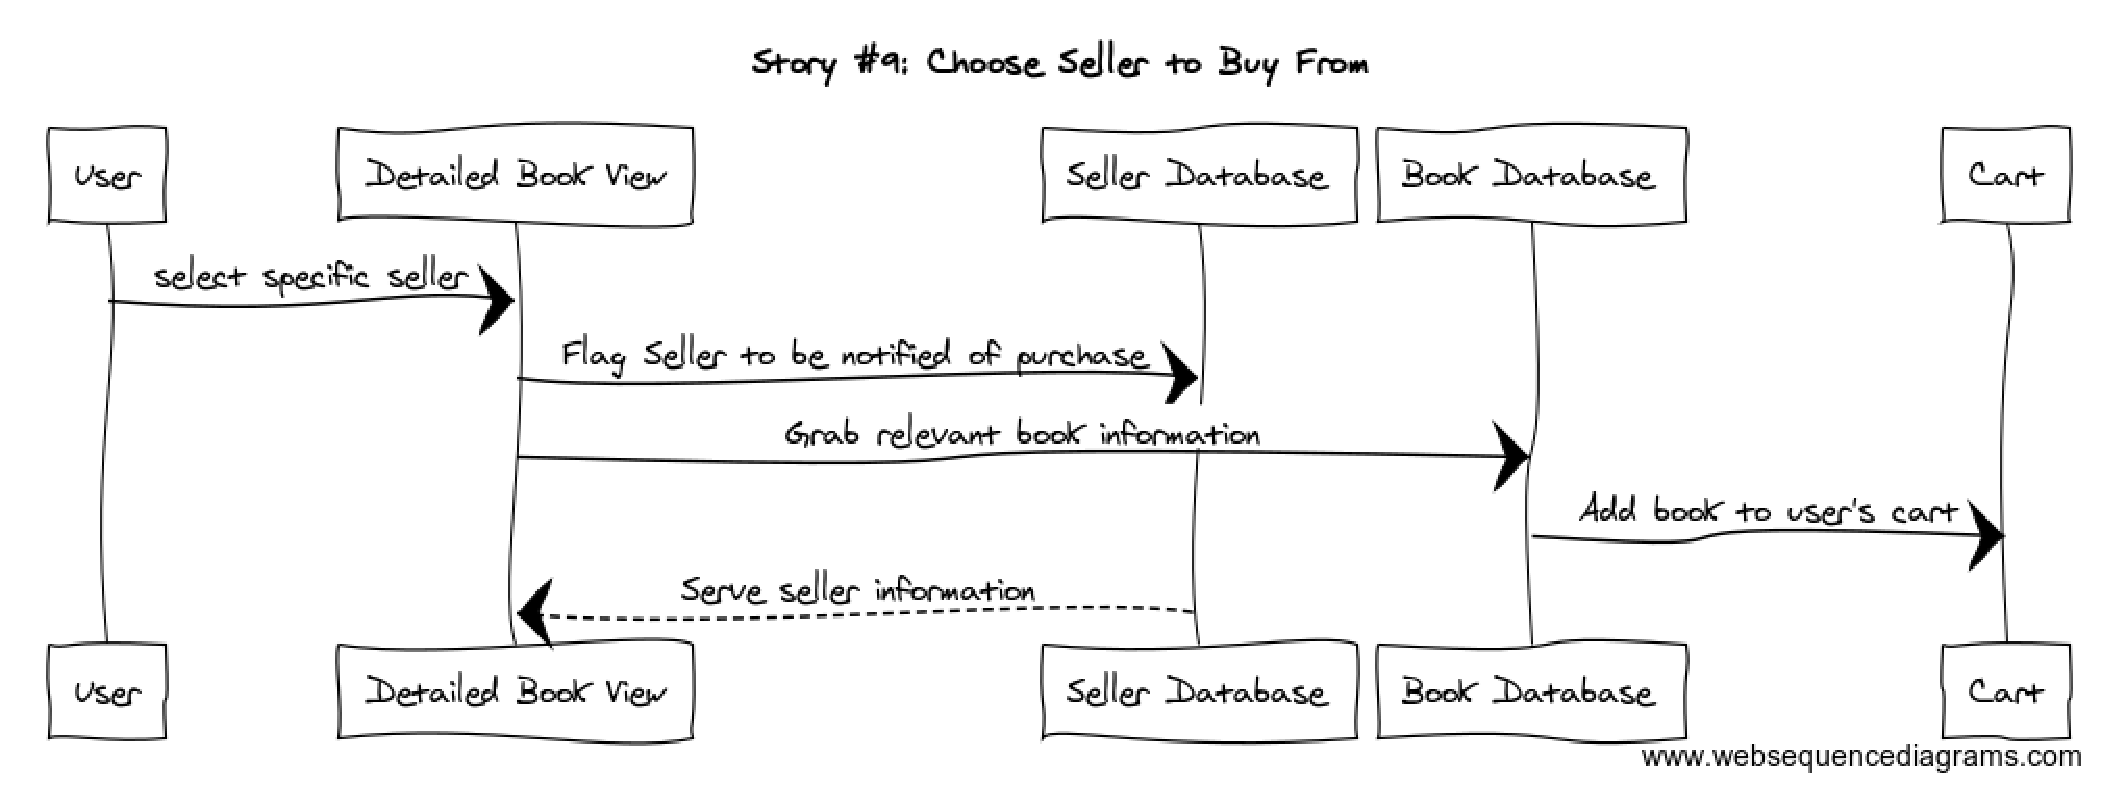
\includegraphics[width=17cm]{story9.eps}
 		%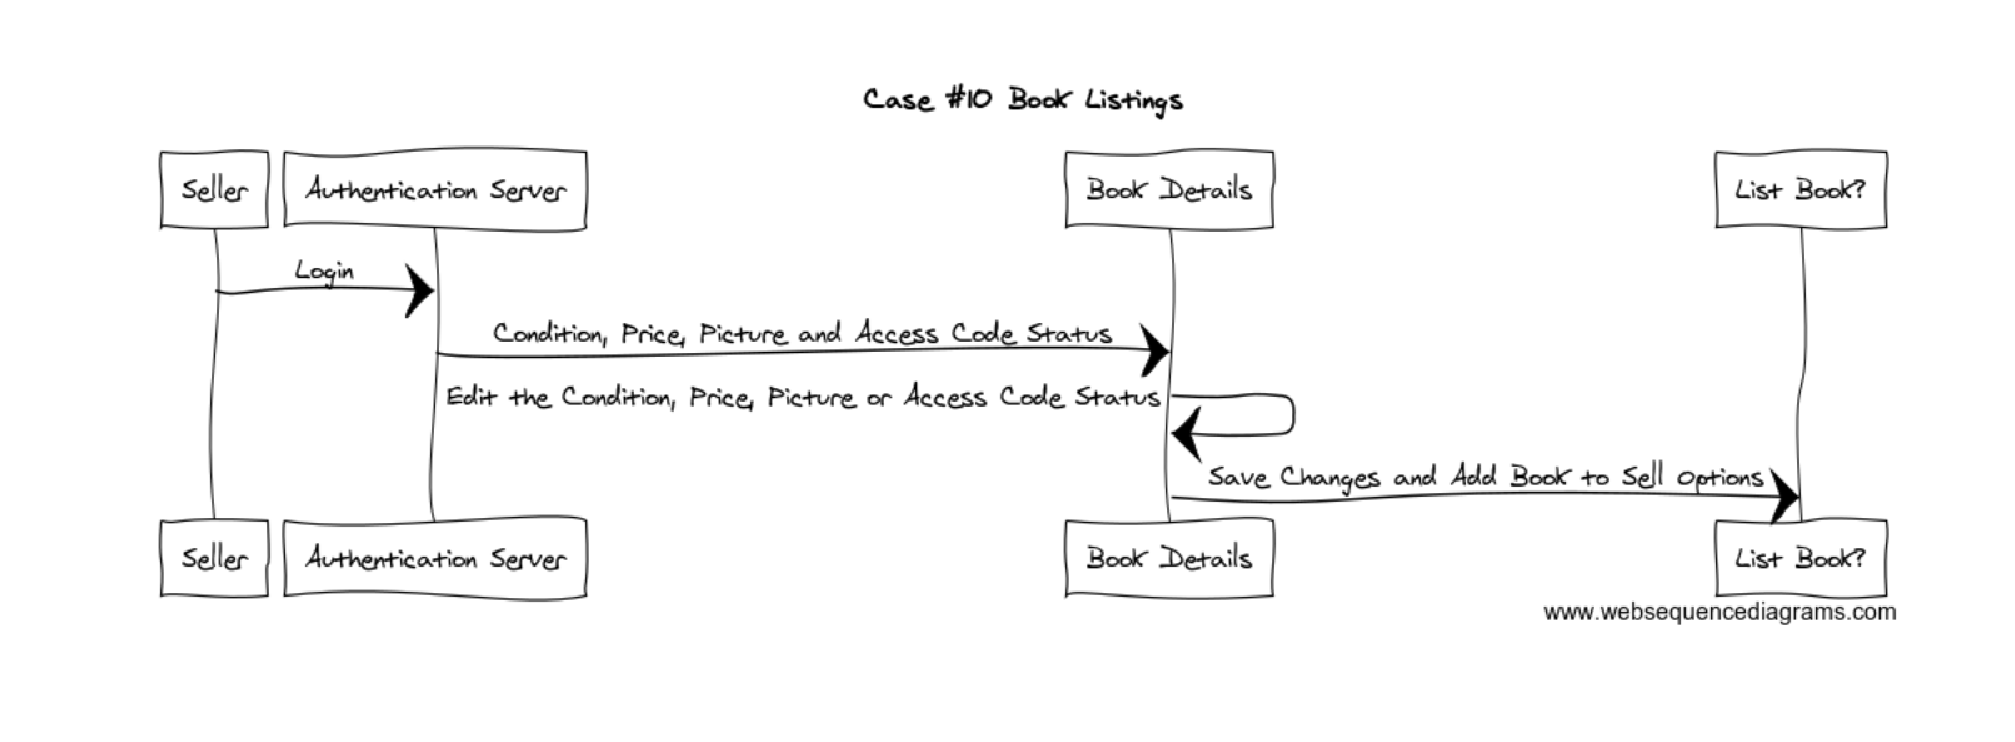
\includegraphics[width=16cm]{story10.eps}
 		%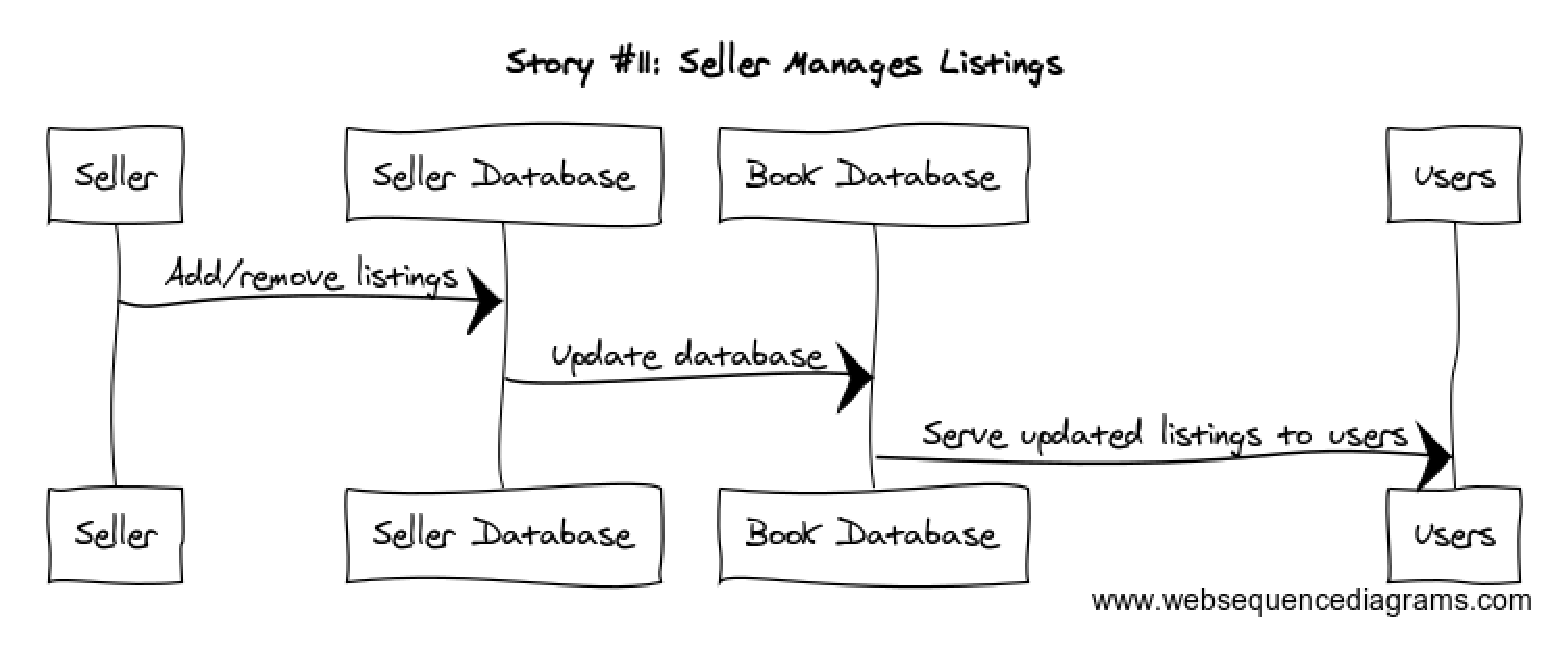
\includegraphics[width=16cm]{story11.eps}

	\section{The Stories due Next Week}
		\begin{itemize}
		\item Story 2: As a User I can add textbooks to the cart so that I can keep track of the books I am interested in.

		\item Story 3: As a User I can remove textbooks I no longer want from the cart.

		\item Story 8: As a User I can select a specific book so that I can view detailed information on it.
		\end{itemize}
		We decided to work on these particular user stories next week because they represent a baseline implementation of our project. 
		Our search and seller user stories are dependent on the existence of a book database and schema for the user to buy books. 
		We will write basic HTML for the main page and get some sample books encoded into our database.
		\subsection{Organization}
		HTML Framework: Cody and Cong \par
		Book Database: Andrew and Jacob \par
		Cart Interface/Record: Mingyu \par

		We should be able to work on the HTML and book database simultaneously. 
		After we have a working implementation of those, then we can get a simple cart interface integrated with them.



	\section{Meeting Report}
		\subsection{Progress Made}
		This week we were able to have everyone come together for our weekly meeting. 
		Together we discussed how we should best divide up the project as well as came up with several user stories that we could utilize. 
		As we worked separately on our tasks, we were sure to keep everyone informed about what we were doing and what our next steps were through our group text. 
		We have continued to use google drive for organizing the differents parts of the project.  

		\subsection{Plans/Goals for Next Week}
		We assume that next weeks project will build further off of this one, but as of yet we have received no information about it. 
		We should have it by friday in which we will get together and discuss what is needed.

		\subsection{Contributions of Each Member}
		\quad User Stories--All Members \par
		UML Sequence Diagrams/Spikes--All Members \par
		Corresponding Tasks--Cong \par
		The Stories due Next Week--Jacob \par
		Meeting Report--Andrew \par
		LaTeX--Jacob

		\subsection{Customer}
		The customer was very helpful with coming up with the user stories that we would use for this project. 
		They agreed with the ones that we were able to come up with as well as helped come up with others.

	\end {document}
	
